% Compile with: 
% cd C:\GusDocs\org\thesis\Gus-thesis\internal-defense\
% pdflatex --shell-escape -synctex=1 -interaction=nonstopmode internal-defense.tex 

\documentclass[presentation]{beamer}
%\usepackage[space]{grffile}
\usepackage[utf8]{inputenc}
\usepackage[T1]{fontenc}
\usepackage[normalem]{ulem}
\usepackage{algorithm, algorithmic, amsfonts, amsmath, amssymb, amsthm, amsbsy, array, babel, booktabs, bm, capt-of, circuitikz, color, float, graphicx, grffile, hyperref, lineno, longtable, mathdots, mathptmx, mathtools, minted, pgf, rotating, subfigure, textcomp, tikz, times, units, verbatim, wrapfig, xcolor} % 
\usepackage[outdir=./]{epstopdf}
\usetikzlibrary{shapes, arrows, calc, patterns, decorations.pathmorphing, decorations.markings, positioning}

%newproof, subcaption, 
%\newtheorem{thm}{Theorem}
%\newtheorem{lem}[thm]{Lemma}
%\newproof{pf}{Proof}

\DeclareMathAlphabet\mathbfcal{OMS}{cmsy}{b}{n}

\input{C:/GusDocs/org/texinputs/mystyle-beamer-org}
\titlegraphic{\includegraphics[width=5cm]{C:/GusDocs/org/texinputs/vublogo/RGB/VUB_logo.pdf}}

% \useinnertheme{circles}
%\setbeamertemplate{itemize items}[circle]
\setbeamertemplate{navigation symbols}{}
\setbeamertemplate{footline}{\hfill \usebeamertemplate***{navigation symbols} \hspace*{0.3cm} \vspace*{0.3cm} \leavevmode \hbox{\begin{beamercolorbox}[wd=0.9\paperwidth,ht=2.25ex,dp=1ex,right]{date in head/foot} \insertframenumber{} \hspace*{1ex} \end{beamercolorbox}} \vskip0pt}
\setbeamerfont{footline}{size=\fontsize{8}{9}}
\addtocounter{framenumber}{0}
\thispagestyle{fancy}
\usetheme{}
\usecolortheme{}

\author{Gustavo Quintana Carapia}
\date{}
\title{Statistical analysis and experimental validation \linebreak of data-driven dynamic measurement methods}

\newcommand\Wider[2][3em]{%
\makebox[\linewidth][c]{%
  \begin{minipage}{\dimexpr\textwidth+#1\relax}
  \raggedright#2
  \end{minipage}%
  }%
}

\begin{document}

\begin{frame}[noframenumbering,plain]
\Wider{\maketitle}
\end{frame}

%\linebreak 

\begin{frame}[label={slide:context}]{A measurement is a dynamic process}
\begin{itemize}
\item The sensor interacts with its environment.
\item The error is inevitably present in the sensor response.
\item The aim is to estimate the input from the sensor response.
\end{itemize}
\begin{figure}[htb!]
\centering
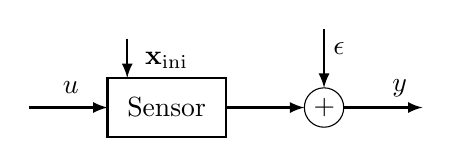
\begin{tikzpicture}[every node/.style={draw,outer sep=0pt,thick}] 
 \node (NB1) [minimum width=1.5cm,minimum height=0.75cm,xshift=0.0cm, yshift=0.0cm] {Sensor};
 \draw [-latex,thick] (NB1.east) ++(0,0) -- +(1.0cm,0);
 \draw [-latex,thick] (NB1.north) ++(-0.5cm,0.5) -- +(0.0cm,-0.5);
 \node[draw=none,fill=none] [above=of NB1,xshift=0.0cm,yshift=-1.0cm] {$\mathbf{x}_{\text{ini}}$};
 \node[draw=none,fill=none] [right=of NB1,xshift=1.0cm,yshift=0.25cm] {${y}$};
 \draw [-latex,thick] (NB1.west) +(-1.0,0) -- +(0.0cm,0);
 \node[draw=none,fill=none] [left=of NB1, xshift=0.750cm,yshift=0.25cm] {${u}$}; 
 \draw (2,0.0) circle (2.5mm);
 \node[draw=none,fill=none] [right=of NB1,xshift=0.00mm,yshift=0.0mm]{+};
 \draw [-latex,thick] (NB1.west) +(3.0,0) -- +(4.0cm,0); 
  \draw [-latex,thick] (NB1.west) ++(2.75cm,1.0) -- +(0.0cm,-0.75);
 \node[draw=none,fill=none] [right=of NB1,xshift=0.250cm,yshift=0.75cm] {$\epsilon$};
\end{tikzpicture}
\end{figure}
%\begin{columns}
%\begin{column}{0.35\columnwidth}
%\begin{block}{}
%\end{block}
%\end{column}
%\begin{column}{0.65\columnwidth}
%\begin{block}{}
%\begin{center}
%\includegraphics[width=.9\linewidth]{./ytilde.eps}
%\end{center}
%\end{block}
%\end{column}
%\end{columns}
\end{frame}

%\begin{frame}[label={slides:have}]{Methods for step input estimation.}
%\begin{columns}
%\begin{column}{0.5\columnwidth}
%\begin{block}{Known model}
%Kalman filter.
%State space recursions.
%\end{block}
%\end{column}
%\begin{column}{0.5\columnwidth}
%\begin{block}{Unknown model}
%Data-driven.
%Local optimization.    
%\end{block}
%\end{column}
%\end{columns}
%\end{frame}

\begin{frame}[label={slide:have}]{A compensator is typically used \linebreak to estimate the input from the sensor response}
\begin{itemize}
\item The additional convolution inverts the sensor dynamics.
\end{itemize}
\begin{figure}[htb!]
\centering
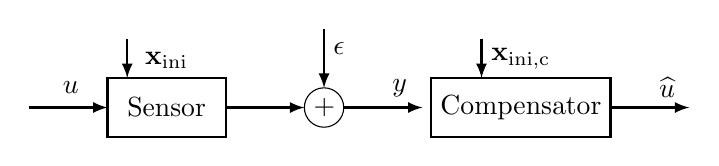
\begin{tikzpicture}[every node/.style={draw,outer sep=0pt,thick}] 
 \node (NB1) [minimum width=1.5cm,minimum height=0.75cm,xshift=0.0cm, yshift=0.0cm] {Sensor};
 \draw [-latex,thick] (NB1.east) ++(0,0) -- +(1.0cm,0);
 \draw [-latex,thick] (NB1.north) ++(-0.5cm,0.5) -- +(0.0cm,-0.5);
 \node[draw=none,fill=none] [above=of NB1,xshift=0.0cm,yshift=-1.0cm] {$\mathbf{x}_{\text{ini}}$};
 \node[draw=none,fill=none] [right=of NB1,xshift=1.0cm,yshift=0.25cm] {${y}$};
 \draw [-latex,thick] (NB1.west) +(-1.0,0) -- +(0.0cm,0);
 \node[draw=none,fill=none] [left=of NB1, xshift=0.750cm,yshift=0.25cm] {${u}$};
 \draw (2,0.0) circle (2.5mm);
 \node[draw=none,fill=none] [right=of NB1,xshift=0.00mm,yshift=0.0mm]{+};
 \draw [-latex,thick] (NB1.west) +(3.0,0) -- +(4.0cm,0); 
  \draw [-latex,thick] (NB1.west) ++(2.75cm,1.0) -- +(0.0cm,-0.75);
 \node[draw=none,fill=none] [right=of NB1,xshift=0.250cm,yshift=0.75cm] {$\epsilon$};
\node (NB2) [minimum width=1.5cm, minimum height=0.75cm, xshift=4.5cm, yshift=0.0cm] {Compensator}; 
 \draw [-latex,thick] (NB2.north) ++(-0.5cm,0.5) -- +(0.0cm,-0.5);
 \node[draw=none,fill=none] [above=of NB2,xshift=0.0cm,yshift=-1.0cm] {$\mathbf{x}_{\text{ini,c}}$};
 \draw [-latex,thick] (NB2.east) ++(0,0) -- +(1.0cm,0);
 \node[draw=none,fill=none] [right=of NB2,xshift=-0.5cm,yshift=0.25cm] {$\widehat{{u}}$};
 \end{tikzpicture}
 \end{figure}
\end{frame}

\begin{frame}[label={slide:have}]{Digital signal processors can help \linebreak to reduce the measurement time even more}
Appropriate DSP programming  can 
\begin{itemize}
\item emulate dynamical systems, or 
\item implement data-driven methods. 
\end{itemize}
\begin{figure}[htb!]
\centering
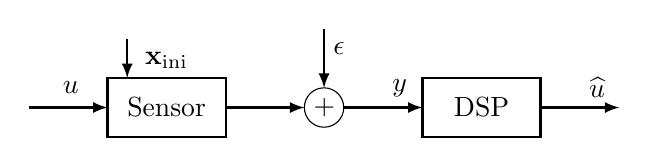
\begin{tikzpicture}[every node/.style={draw,outer sep=0pt,thick}] 
 \node (NB1) [minimum width=1.5cm,minimum height=0.75cm,xshift=0.0cm, yshift=0.0cm] {Sensor};
 \draw [-latex,thick] (NB1.east) ++(0,0) -- +(1.0cm,0);
 \draw [-latex,thick] (NB1.north) ++(-0.5cm,0.5) -- +(0.0cm,-0.5);
 \node[draw=none,fill=none] [above=of NB1,xshift=0.0cm,yshift=-1.0cm] {$\mathbf{x}_{\text{ini}}$};
 \node[draw=none,fill=none] [right=of NB1,xshift=1.0cm,yshift=0.25cm] {${y}$};
 \draw [-latex,thick] (NB1.west) +(-1.0,0) -- +(0.0cm,0);
 \node[draw=none,fill=none] [left=of NB1, xshift=0.750cm,yshift=0.25cm] {${u}$};
 \draw (2,0.0) circle (2.5mm);
 \node[draw=none,fill=none] [right=of NB1,xshift=0.00mm,yshift=0.0mm]{+};
 \draw [-latex,thick] (NB1.west) +(3.0,0) -- +(4.0cm,0); 
  \draw [-latex,thick] (NB1.west) ++(2.75cm,1.0) -- +(0.0cm,-0.75);
 \node[draw=none,fill=none] [right=of NB1,xshift=0.250cm,yshift=0.75cm] {$\epsilon$};
\node (NB2) [minimum width=1.5cm, minimum height=0.75cm, xshift=4.0cm, yshift=0.0cm] {DSP}; 
 \draw [-latex,thick] (NB2.east) ++(0,0) -- +(1.0cm,0);
 \node[draw=none,fill=none] [right=of NB2,xshift=-0.5cm,yshift=0.25cm] {$\widehat{{u}}$};
 \end{tikzpicture}
 \end{figure}
\end{frame}

\begin{frame}[label={slide:have}]{In this work we focus on a data-driven \linebreak step input estimation method}
\begin{itemize}
\item The method is formulated as a structured and correlated errors-in-variables problem. 
\item The online solution is computed using recursive least squares. 
\end{itemize}
\end{frame}

\begin{frame}[label={slide:need}]{The uncertainty of the data-driven step input estimation method was unknown}
\begin{itemize}
\item The validation of the method was necessary to foster \linebreak the method utilization in metrology applications. 
\end{itemize}
\end{frame}

\begin{frame}[label={slide:objective}]{A statistical analysis was conducted to find the data-driven step input estimation method uncertainty}
\begin{itemize}
\item This analysis unveils the step input estimation mean and variance, and thus, the method uncertainty.  
\item The estimation mean and variance knowledge permits to evaluate the method and its effectiveness. 
\end{itemize}
\end{frame}


\begin{frame}[label={slide:plan}]{The conducted research work covered}
\begin{enumerate}
\item A statistical analysis of structured and correlated errors-in-variables problems. 
\item An experimental validation based on the uncertainty of \linebreak the step input estimation method. 
\item The proposal of two affine input estimation methods. 
\end{enumerate}
\end{frame}

\begin{frame}[label={slide:preliminaries1}]{To formulate the input estimation methods, we consider a measurement is a linear system problem}
\begin{figure}[htb!]
\centering
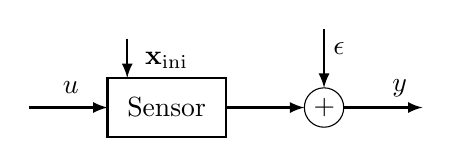
\begin{tikzpicture}[every node/.style={draw,outer sep=0pt,thick}] 
 \node (NB1) [minimum width=1.5cm,minimum height=0.75cm,xshift=0.0cm, yshift=0.0cm] {Sensor};
 \draw [-latex,thick] (NB1.east) ++(0,0) -- +(1.0cm,0);
 \draw [-latex,thick] (NB1.north) ++(-0.5cm,0.5) -- +(0.0cm,-0.5);
 \node[draw=none,fill=none] [above=of NB1,xshift=0.0cm,yshift=-1.0cm] {$\mathbf{x}_{\text{ini}}$};
 \node[draw=none,fill=none] [right=of NB1,xshift=1.0cm,yshift=0.25cm] {${y}$};
 \draw [-latex,thick] (NB1.west) +(-1.0,0) -- +(0.0cm,0);
 \node[draw=none,fill=none] [left=of NB1, xshift=0.750cm,yshift=0.25cm] {${u}$}; 
 \draw (2,0.0) circle (2.5mm);
 \node[draw=none,fill=none] [right=of NB1,xshift=0.00mm,yshift=0.0mm]{+};
 \draw [-latex,thick] (NB1.west) +(3.0,0) -- +(4.0cm,0); 
  \draw [-latex,thick] (NB1.west) ++(2.75cm,1.0) -- +(0.0cm,-0.75);
 \node[draw=none,fill=none] [right=of NB1,xshift=0.250cm,yshift=0.75cm] {$\epsilon$};
\end{tikzpicture}
\end{figure}
\begin{itemize}
\item  With LTI sensor, the measurement dynamics \linebreak can be described using state-space representation: 
\end{itemize}
\begin{equation*} \begin{aligned} \mathbf{x}(k+1) &= \mathbf{A} \mathbf{x}(k) + \mathbf{B} {u}(k), \quad \text{with} \quad \mathbf{x}_{\text{ini}} = \mathbf{x}(0) \\ 
{y}(k) &= \mathbf{C} \mathbf{x}(k) + {D} {u}(k) + {\epsilon}(k) \end{aligned} \end{equation*}
\end{frame}

\begin{frame}[label={slide:preliminaries2}]{If the sensor model and initial conditions are known, and we have the exact data sensor response}
\begin{itemize}
\item  then, the input can be estimated from: 
\end{itemize}
\begin{equation*} 
\underbrace{ \begin{bmatrix} y(0) \\ y(1) \\ y(2) \\ \vdots \\ y(T) \end{bmatrix} }_{\mathbf{y}}
 = \underbrace{ \begin{bmatrix} \mathbf{C} \\ \mathbf{C} \mathbf{A} \\ \mathbf{C} \mathbf{A}^2 \\ \vdots \\ \mathbf{C} \mathbf{A}^T \end{bmatrix} }_{\mathbfcal{O}} \mathbf{x}(0) +
 \underbrace{ \begin{bmatrix} \mathbf{D} \\ \mathbf{C} \mathbf{B} & \mathbf{D} \\ \mathbf{C} \mathbf{A} \mathbf{B} & \mathbf{C} \mathbf{B} & \mathbf{D} \\ \vdots & \ddots \\ \mathbf{C} \mathbf{A}^{T-1} \mathbf{B} & \cdots  &  \mathbf{C} \mathbf{A} \mathbf{B} & \mathbf{C} \mathbf{B} & \mathbf{D} \end{bmatrix} }_{\mathbfcal{T}} \underbrace{ \begin{bmatrix} u(0) \\ u(1) \\ u(2) \\ \vdots \\ u(T) \end{bmatrix} }_{\mathbf{u}} \end{equation*}
\end{frame}

\begin{frame}[label={slide:preliminaries3}]{A step input ${u} = \bar{{u}} s$ permits a representation \linebreak with an augmented state space }
\begin{itemize}
\item The step input adds a pole at (1,0) to the original system: 
\end{itemize}
\begin{equation*} \begin{aligned} \mathbf{x}_\text{a}(k+1) &= \underbrace{ \begin{bmatrix} \mathbf{A} & \mathbf{B} \\ 0 & 1 \end{bmatrix} }_{\mathbf{A}_\text{a}} \mathbf{x}_\text{a}(k) , \quad \text{where} \ \ \mathbf{x}_\text{a}(k) = \begin{bmatrix} \mathbf{x}(k) \\ {u}(k) \end{bmatrix}, \ \ \mathbf{x}_{\text{ini}} = \mathbf{x}(0) \\
{y}(k) &= \underbrace{ \begin{bmatrix} \mathbf{C} & D \end{bmatrix} }_{\mathbf{C}_\text{a}} \mathbf{x}_\text{a}(k) \end{aligned} \end{equation*}
\end{frame}

\begin{frame}[label={slide:preliminaries4}]{Without sensor model, one alternative to estimate the step input  starts by formulating}
\small
\begin{equation*} \begin{aligned} & \underbrace{ \begin{bmatrix} y(1) & y(2) & \cdots & y(n) \\ y(2) & y(3) & \cdots & y(n+1) \\ \iddots & \iddots & \iddots \\ y(n) & y(n+1) & \cdots & y(2n-1) \end{bmatrix} }_{ \mathbfcal{H}({y}) } = \underbrace{ \begin{bmatrix} \widehat{\mathbf{C}}_\text{a} \\ \widehat{\mathbf{C}}_\text{a} \widehat{\mathbf{A}}_\text{a} \\ \vdots \\ \widehat{\mathbf{C}}_\text{a} \widehat{\mathbf{A}}_\text{a}^{n} \end{bmatrix} }_{ \mathbfcal{O}_\text{a} }  \underbrace{ \begin{bmatrix} \mathbf{x}_\text{a}(0) & \mathbf{x}_\text{a}(1) & \cdots & \mathbf{x}_\text{a}(n) \end{bmatrix} }_{ \mathbf{X}_\text{ini} } \end{aligned} \end{equation*}
\normalsize
 A singular value decomposition of $\mathbfcal{H}({y})$ permits the estimation of the observability matrix $\mathbfcal{O}_\text{a}$ and the initial conditions $\mathbf{X}_\text{ini}$ \nolinebreak
\begin{equation*}  \widehat{\mathbfcal{O}}_\text{a} = \mathbf{U} \sqrt{\bm{\Sigma}} \quad \mathrm{and} \quad \widehat{\mathbf{X}}_\text{ini} = \sqrt{\bm{\Sigma}} \mathbf{V}n, \quad \mathrm{from} \quad \mathbf{U} \bm{\Sigma} \mathbf{V} = \mathbfcal{H}({y}) \end{equation*}
\end{frame}

\begin{frame}[label={slide:preliminaries5}]{Once we have estimated the observability matrix $\mathbfcal{O}_\text{a}$ and the initial conditions $\mathbf{X}_\text{ini}$, we can write}
\begin{equation*}  {y} = G \ \bar{{u}} \ + \ \widehat{\mathbfcal{O}}_\text{a} \ \mathbf{x}_\text{a}(0) , \end{equation*}
\begin{itemize}
\item that is equivalent to: 
%\begin{equation*}  \underbrace{ \begin{bmatrix}y(0) \\ y(1) \\ \vdots \\ y(T) \end{bmatrix}}_{\mathbf{y}} = \underbrace{ \begin{bmatrix} G & \mathbf{C}_\text{a} \\ G & \mathbf{C}_\text{a} \mathbf{A}_\text{a} \\ \vdots & \vdots \\ G & \mathbf{C}_\text{a} \mathbf{A}_\text{a}^T \end{bmatrix}}_{\mathbf{K}} \begin{bmatrix} \bar{{u}} \\ \mathbf{x}_\text{a}(0) \end{bmatrix} \end{equation*}
\begin{equation*}  \underbrace{ \begin{bmatrix}y(0) \\ \vdots \\ y(T) \end{bmatrix}}_{\mathbf{y}} = \underbrace{ \begin{bmatrix} G \otimes \mathbf{1}_{T+1} & \widehat{\mathbfcal{O}}_\text{a} \end{bmatrix}}_{\mathbf{K}} \begin{bmatrix} \bar{{u}} \\ \mathbf{x}_\text{a}(0) \end{bmatrix} \end{equation*}
\item and admits a least-squares solution
\begin{equation*}  \begin{bmatrix} \widehat{{u}} \\ \widehat{\mathbf{x}}_{\text{ini}} \end{bmatrix} = \left( \mathbf{K}^\top \mathbf{K} \right)^{-1} \mathbf{K}^\top \mathbf{y} \end{equation*}
\end{itemize}
\end{frame}

\begin{frame}[label={slide:preliminaries6}]{Another alternative to estimate the step input \linebreak starts by differentiating the state-space representation} 
\begin{equation*} \begin{aligned} \Delta \mathbf{x}(k+1) = \mathbf{A} \Delta \mathbf{x}(k), \quad \Delta {y}(k) = \mathbf{C} \Delta \mathbf{x}(k), \quad \text{with} \quad \Delta \mathbf{x}_{\text{ini}} = \Delta \mathbf{x}(0) \end{aligned} \end{equation*}
\begin{columns}
\begin{column}{0.35\columnwidth}
where: \linebreak $\Delta = \sigma - 1$, and \linebreak $(\sigma^\tau y) (k) = y(k + \tau)$.
\end{column}
\begin{column}{0.65\columnwidth}
If $\Delta {y}$ is persistently exciting of order $L$, 
\begin{equation*} \mathrm{rank} \left( \mathbfcal{H}_{L+1} \left( \Delta {y} \right) \right) \leq L  \end{equation*} 
\end{column}
\end{columns}
\linebreak 
then, we can write the total response of the system as  
%\begin{equation*} \mathbf{y} = G \bar{u} + \mathbfcal{H}\left(\Delta {y}\right) \bm{\ell} \end{equation*}
%that is equivalent to
%\begin{equation*} \underbrace{ \begin{bmatrix} y(n+1) \\ \vdots \\ y(T) \end{bmatrix}}_{\mathbf{y}} = \underbrace{ \begin{bmatrix} G & \Delta y(1) & \Delta y(2) & \cdots & \Delta y(n) \\ G & \Delta y(2) & \Delta y(3) & \cdots & \Delta y(n+1) \\ \vdots & \iddots & \iddots & \iddots \\ G & \Delta y(T-n) & \Delta y(T-n+1) & \cdots & \Delta y(T-1) \end{bmatrix}}_{\mathbf{K}} \underbrace{ \begin{bmatrix} \bar{{u}} \\ \bm{\ell} \end{bmatrix} }_{\bm{\theta}} \end{equation*}
\begin{equation*} \underbrace{ \begin{bmatrix} y(n+1) \\ \vdots \\ y(T) \end{bmatrix}}_{\mathbf{y}} = \underbrace{ \begin{bmatrix} G \otimes \mathbf{1}_{T+1} & \mathbfcal{H}\left(\Delta {y}\right) \end{bmatrix}}_{\mathbf{K}} \underbrace{ \begin{bmatrix} \bar{{u}} \\ \bm{\ell} \end{bmatrix} }_{\bm{\theta}} \end{equation*}
\end{frame}

\begin{frame}[label={slide:preliminaries7}]{The data-driven step input estimation method is a structured and correlated errors-in-variables problem}
considering the addition of the measurement noise
\begin{equation*} \begin{aligned} \widetilde{\mathbf{y}} &= \mathbf{y} + \bm{\epsilon} , \\
\widetilde{\mathbf{K}} &= \mathbf{K} + \mathbf{E} , \end{aligned} \end{equation*}
we have
\begin{equation*} \underbrace{ \begin{bmatrix} \widetilde{y}(n+1) \\ \vdots \\ \widetilde{y}(T) \end{bmatrix}}_{\widetilde{\mathbf{y}}} = \underbrace{ \begin{bmatrix} G \otimes \mathbf{1}_{T+1} & \mathbfcal{H}\left(\Delta {\widetilde{y}}\right) \end{bmatrix}}_{\widetilde{\mathbf{K}}} \underbrace{ \begin{bmatrix} \bar{{u}} \\ \bm{\ell} \end{bmatrix} }_{\bm{\theta}} \end{equation*}
%and  $\mathbf{E}$ is constructed with the noise data
%\begin{equation*} \mathbf{E} = \begin{bmatrix} 0 & \Delta \epsilon(1) & \Delta \epsilon(2) & \cdots & \Delta \epsilon(n) \\ 0 & \Delta \epsilon(2) & \Delta \epsilon(3) & \cdots & \Delta \epsilon(n+1) \\ \vdots & \vdots & \vdots & & \vdots \\ 0 & \Delta \epsilon(T-n) & \Delta \epsilon(T-n+1) & \cdots & \Delta \epsilon(T-1) \end{bmatrix} \end{equation*}
\end{frame}

\begin{frame}[label={slide:statistical1}]{What are the statistical moments of the least-squares solution of a structured and correlated errors-in-variables problem?}
\begin{equation*} \widehat{\bm{\theta}} = \widetilde{\mathbf{K}}^\dagger \widetilde{\mathbf{y}} = ( \widetilde{\mathbf{K}}^\top \widetilde{\mathbf{K}} )^{-1} \widetilde{\mathbf{K}}^\top \widetilde{\mathbf{y}} \end{equation*}
\end{frame}

\begin{frame}[label={slide:statistical1_2}]{Since the noise is assumed additive}
\begin{equation*} \begin{aligned} \widehat{\bm{\theta}} &= \left( (\mathbf{K}+\mathbf{E})^\top (\mathbf{K}+\mathbf{E})  \right)^{-1} (\mathbf{K}+\mathbf{E})^\top (\mathbf{y}+\bm{\epsilon}) \\
&= \left( \mathbf{I} + \mathbf{M} \right)^{-1} \mathbf{Q}^{-1} (\mathbf{K}+\mathbf{E})^\top (\mathbf{y}+\bm{\epsilon}) \end{aligned}\end{equation*} 
\linebreak 
where
\begin{equation*} \begin{aligned}  \mathbf{Q} &= \mathbf{K}^\top \mathbf{K}, \quad \text{and} \\
\quad \mathbf{M} &= \mathbf{Q}^{-1} ( \mathbf{K}^\top \mathbf{E} + \mathbf{E}^\top \mathbf{K} + \mathbf{E}^\top \mathbf{E} ). \end{aligned} \end{equation*} 
\end{frame}

\begin{frame}[label={slide:statistical2}]{A second order Taylor series aproximation of the inverse matrix permits to study the LS solution}
Using
\begin{equation*} (\mathbf{I} + \mathbf{M})^{-1} \approx \mathbf{I} - \mathbf{M} + \mathbf{M}^2, \end{equation*} 
the LS solution is approximated by
\begin{equation*} \widehat{\bm{\theta}} \approx \left( \mathbf{I} - \mathbf{M} + \mathbf{M}^2 \right) \mathbf{Q}^{-1} (\mathbf{K}+\mathbf{E})^\top (\mathbf{y}+\bm{\epsilon}) \end{equation*} 
\linebreak
To find the LS solution bias and covariance, we use
\begin{equation*} \begin{aligned} \bm{\mu} \left(\widehat{\bm{\theta}} \right) &= \mathbb{E} \left\{ \widehat{\bm{\theta}} \right\}, \quad \mathbf{b} \left(\widehat{\bm{\theta}} \right) = \bm{\mu}\left(\widehat{\bm{\theta}} \right) - \bm{\theta} \\
\mathbf{C} \left( \widehat{\bm{\theta}} \right) &= \mathbb{E} \left\{ \left( \widehat{\bm{\theta}} - \bm{\mu} \right) \left( \widehat{\bm{\theta}} - \bm{\mu} \right)^\top \right\} . \end{aligned} \end{equation*} 
\end{frame}

\begin{frame}[label={slide:statistical3}]{For an unstructured and uncorrelated EIV problem, the bias and covariance of the LS solution are}
\begin{equation*} \begin{aligned} \mathbf{b}_{\mathrm{p}} \left( \widehat{\bm{\theta}} \right) & \approx \sigma_{\mathbf{E}}^2 \left( 2 + 2n - T \right) \mathbf{Q}^{-1} \bm{\theta} \\
\\
\mathbf{C}_{\mathrm{p}} \left( \widehat{\bm{\theta}} \right) & \approx \sigma_{\bm{\epsilon}}^2 \ \mathbf{Q}^{-1} + \sigma_{\mathbf{E}}^2 \ \mathrm{trace} \left( \bm{\theta} \bm{\theta}^\top \right) \mathbf{Q}^{-1} \\
\quad & - \sigma_{\mathbf{E}}^4 \left( 2 + 2n - T \right)^2 \ \mathbf{Q}^{-1} \bm{\theta} \bm{\theta}^\top \mathbf{Q}^{-1}  \end{aligned} \end{equation*}
\end{frame}

\begin{frame}[label={slide:statistical4}]{It is proposed to substitute the observed variables in the derived expressions.}
The observed variables are $\widetilde{\mathbf{y}}$, $\widetilde{\mathbf{K}}$, and from them we compute $\widehat{\bm{\theta}}$.
The substitution gives an approximation of the estimation bias and covariance using the observed data.
\begin{equation*} \begin{aligned} \widetilde{\mathbf{b}}_{\mathrm{p}} \left( \widehat{\bm{\theta}} \right) & \approx \sigma_{\mathbf{E}}^2 \left( 2 + 2n - T \right) \widetilde{\mathbf{Q}}^{-1} \widehat{\bm{\theta}} \\
\\
\widetilde{\mathbf{C}}_{\mathrm{p}} \left( \widehat{\bm{\theta}} \right) & \approx \sigma_\epsilon^2 \ \widetilde{\mathbf{Q}}^{-1} + \sigma_{\mathbf{E}}^2 \ \mathrm{trace} \left( \widehat{\bm{\theta}} \widehat{\bm{\theta}}^\top \right) \widetilde{\mathbf{Q}}^{-1} \\
&\quad - \sigma_{\mathbf{E}}^4 \left( 2 + 2n - T \right)^2 \widetilde{\mathbf{Q}}^{-1} \widehat{\bm{\theta}} \widehat{\bm{\theta}}^\top \widetilde{\mathbf{Q}}^{-1} \end{aligned} \end{equation*}
\end{frame}

\begin{frame}[label={slide:statistical5}]{For the structured and correlated EIV problem in the data-driven step input estimation method}
the bias and covariance of the LS solution are
\begin{equation*} \begin{aligned} \mathbf{b}_{\mathrm{p}} \left( \widehat{\bm{\theta}} \right) & \approx \mathbf{Q}^{-1} \left( \left( \mathbf{K}^\top \mathbf{B}_1 - \mathbf{B}_2 \right) \mathbf{x} - \left( \mathbf{K}^\top \mathbf{B}_3 - \mathbf{B}_4 \right) \right) \\ \\
\mathbf{C}_{\mathrm{p}} \left( \widehat{\bm{\theta}} \right) & \approx \mathbf{K}^\dagger \left( \sigma_{\bm{\epsilon}}^2 \mathbf{I}_{T-n} + \mathbf{C}_1 - \mathbf{C}_2 - \mathbf{C}_2^\top \right) \mathbf{K}^{\dagger \top} - \mathbf{b}_{\mathrm{p}} \left( \widehat{\bm{\theta}} \right) \mathbf{b}_{\mathrm{p}}^\top \left( \widehat{\bm{\theta}} \right)  \end{aligned} \end{equation*}
where the matrices $\mathbf{B}_1$ to $\mathbf{B}_1$, and $\mathbf{C}_1$ to $\mathbf{C}_2$ can be obtained considering the structure and correlation of the problem.] 
\end{frame}

\begin{frame}[label={slide:statistical6}]{The substitution of the observed variables in the expressions also approximates the estimation bias and covariance}
\begin{equation*} \begin{aligned} \mathbf{b}_{\widetilde{\mathrm{p}}} \left( \widehat{\bm{\theta}} \right) & \approx \widetilde{\mathbf{Q}}^{-1} \left( \left( \widetilde{\mathbf{K}}^\top \widetilde{\mathbf{B}}_1 - \widetilde{\mathbf{B}}_2 \right) \widehat{\bm{\theta}} - \left( \widetilde{\mathbf{K}}^\top \widetilde{\mathbf{B}}_3 - \widetilde{\mathbf{B}}_4 \right) \right) \\ \\
\mathbf{C}_{\widetilde{\mathrm{p}}} \left( \widehat{\bm{\theta}} \right) & \approx \widetilde{\mathbf{K}}^\dagger \left( \sigma_{\bm{\epsilon}}^2 \mathbf{I}_{T-n} + \widetilde{\mathbf{C}}_1 - \widetilde{\mathbf{C}}_2 - \widetilde{\mathbf{C}}_2^\top \right) \widetilde{\mathbf{K}}^{\dagger \top} - \mathbf{b}_{\widetilde{\mathrm{p}}} \left( \widehat{\bm{\theta}} \right) \mathbf{b}_{\widetilde{\mathrm{p}}}^\top \left( \widehat{\bm{\theta}} \right) \end{aligned} \end{equation*}
\end{frame}

\begin{frame}[label={slide:statistical7}]{We can find the Cram\'er-Rao lower bound of the structured and correlated errors-in-variables problem}
It is the lower limit on the estimation variance.
\begin{equation*} \text{CRLB}(\bm{\theta}) = \left( \mathbf{I} + \frac{\partial \mathbf{b} (\widehat{\bm{\theta}}) }{\partial (\widehat{\bm{\theta}})} \right)^\top \mathbf{Fi}^{-1}(\bm{\theta}) \left( \mathbf{I} + \frac{\partial \mathbf{b} (\widehat{\bm{\theta}}) }{\partial (\widehat{\bm{\theta}})} \right) \end{equation*}
Where the Fisher information matrix is  
\begin{equation*} \mathbf{Fi}(x) = - \mathbb{E} \left\{ \frac{\partial ^2 l (\widehat{\bm{\theta}}) }{\partial \widehat{\bm{\theta}}^2 } \right\} \end{equation*}
\end{frame}

\begin{frame}[label={slide:statistical7_2}]{The structured EIV problem can be expressed as a linear in the measurements problem}

\begin{equation*} e (\widehat{\bm{\theta}}, \widetilde{\mathbf{z}}) = \mathbf{M}_1( \widehat{\bm{\theta}} ) \ \widetilde{\mathbf{z}} = \begin{bmatrix} \mathbf{I}_{T-n} & - \widehat{\bm{\theta}}^T \otimes \mathbf{I}_{T-n} \end{bmatrix} \begin{bmatrix} \widetilde{\mathbf{y}} \\ \mathrm{vec} ( \widetilde{\mathbf{K}} ) \end{bmatrix} = 0 .  \end{equation*}
where $\widetilde{\mathbf{z}} = \mathbf{z} + \epsilon_{\mathbf{z}}$, and $\mathbf{C}_{\mathbf{z}}$ is the covariance matrix of $\epsilon_{\mathbf{z}}$. 

Then, the loglikelihood function is
\begin{equation*} \ln{ l(\widetilde{\mathbf{z}}, \widehat{\mathbf{z}}, \widehat{\bm{\theta}}) } = - \frac{1}{2} \left( \widetilde{\mathbf{z}} - \widehat{\mathbf{z}} \right)^\top \mathbf{C}_{\mathbf{z}}^{-1} \left( \widetilde{\mathbf{z}} - \widehat{\mathbf{z}} \right) + \mathrm{constant}, \end{equation*}
and the Fisher information matrix is
\begin{equation*} \mathbf{Fi}(\bm{\theta}) = \left( \frac{\partial e (\widehat{\bm{\theta}}, \mathbf{z}) }{\partial \bm{\theta} } \right)^\top \left( \mathbf{M}_1( \bm{\theta} ) \ \mathbf{C}_{\mathbf{z}} \ \mathbf{M}_1^\top( \bm{\theta} ) \right)^{-1} \left( \frac{\partial e (\widehat{\bm{\theta}}, \mathbf{z}) }{\partial \bm{\theta} } \right) 
 \end{equation*}
\end{frame}

\begin{frame}[label={slide:statistical8}]{Simulation results for unstructured (top) and \linebreak structured EIV problems (bottom)}
\begin{itemize}
\item The absolute value of the bias and the standard error are proportional to the noise variance and standard deviation.
\item The bias predictions coincide with the empirical bias, and 
\item the standard errors are smaller than the estimation bias.
\end{itemize}
\begin{figure}[htb!]
\centering
\includegraphics[width=0.55\columnwidth]{./fig/Stat_Fig_1.pdf} 
\end{figure}
\end{frame}

\begin{frame}[label={slide:statistical9}]{The relative errors of the bias and variance estimation show the accuracy of the derived expressions}
\begin{itemize}
\item The empirical results are closely approximated 
%for unstructured (top) and structured EIV problems (bottom)
\end{itemize}
\begin{figure}[htb!]
\centering
\includegraphics[width=1\columnwidth]{./fig/Stat_Fig_2.pdf} 
\end{figure}
\end{frame}

\begin{frame}[label={slide:statistical10}]{The MSE of the step input estimation is larger than its CRLB at most by one order of magnitude}
\begin{figure}[htb!]
\centering
\includegraphics[width=0.55\columnwidth]{./fig/Stat_Fig_3.pdf} 
\includegraphics[width=0.55\columnwidth]{./fig/Stat_Fig_4.pdf} 
\end{figure}
\end{frame}

\begin{frame}[label={slide:statistical11}]{Observations of the statistical analysis}
\begin{itemize}
\item The predictions in the structured case are more susceptible to perturbations.
\item The bias and variance predictions accuracy depend on the Taylor series validity.
\item This methodology can be applied to assess the uncertainty to other structured EIV problems solutions.
\item The bias and variance expressions obtained depend on each specific structure.
\end{itemize}
\end{frame}

\begin{frame}[label={slide:experimental-validation1}]{A description of the experimental validation of the step input estimation method}
The diagram represents the setup used to measure mass. 
\begin{figure}[htb!]
\centering
\includegraphics[width=0.55\columnwidth]{./fig/Exp_Fig_5.pdf} 
\end{figure}
\end{frame}

\begin{frame}[label={slide:experimental-validation2}]{The step input estimation by processing a simulated (left) and an measured (right) sensor response}
A model of the sensor was obtained using the system identification toolbox.
\begin{figure}[htb!]
\centering
\includegraphics[width=1\columnwidth]{./fig/Exp_Fig_1.pdf} 
\end{figure}
\end{frame}

\begin{frame}[label={slide:experimental-validation3}]{The bias and variance estimation estimation results allow to evaluate the effectiveness with respect to SNR}
In simulation, with an order $n=5$ the SNR region of validity is largar then 40 dB. 
\begin{figure}[htb!]
\centering
\includegraphics[width=0.55\columnwidth]{./fig/Exp_Fig_2.pdf} 
\includegraphics[width=0.55\columnwidth]{./fig/Exp_Fig_3.pdf} 
\end{figure}
\end{frame}

\begin{frame}[label={slide:experimental-validation4}]{The uncertainty of the step input estimation does not decrease for larger order $n$}
\begin{figure}[htb!]
\centering
\includegraphics[width=0.55\columnwidth]{./fig/Exp_Fig_4.pdf} 
\end{figure}
\end{frame}

\begin{frame}[label={slide:experimental-validation5}]{The empirical and the estimation of the bias and variance of the step input for different sample size}
These results are the average from 100 experiments. 
\begin{figure}[htb!]
\centering
\includegraphics[width=0.55\columnwidth]{./fig/Exp_Fig_8.pdf} 
\includegraphics[width=0.55\columnwidth]{./fig/Exp_Fig_11.pdf} 
\end{figure}
\end{frame}

\begin{frame}[label={slide:experimental-validation6}]{The measurement noise contains frequency components characteristic of mechanical systems}
\begin{figure}[htb!]
\centering
\includegraphics[width=0.55\columnwidth]{./fig/Exp_Fig_7.pdf} 
\includegraphics[width=0.55\columnwidth]{./fig/Exp_Fig_9.pdf} 
\end{figure}
\end{frame}

\begin{frame}[label={slide:experimental-validation7}]{The uncertainty of the step input estimation does not depend on the order $n$}
\begin{figure}[htb!]
\centering
\includegraphics[width=0.55\columnwidth]{./fig/Exp_Fig_12.pdf} 
\end{figure}
\end{frame}

\begin{frame}[label={slide:experimental-validation8}]{Observations of the experimental validation of the step input estimation method}
\begin{itemize}
\item In simulation, the input estimation MSE is close to the CRLB theoretical minimum for biased estimators.
\item The step input estimation method is useful in practical applications where the whiteness assumption of the measurement noise is not fulfilled. 
\item The noise variance obtained from the sensor steady state response underestimates the measurement noise variance.
\item Using the predictions, the uncertainty assessment is provided for given sample size and noise variance.
\end{itemize}

\end{frame}


\begin{frame}[label={slide:affine-input-estimation1}]{When an affine input $u=at+b$ is applied to weighing system, it becomes time varying}
\begin{figure}[htb!]
\centering
\includegraphics[width=0.3\columnwidth]{./fig/Aff_Fig_1.pdf} 
\end{figure}
\begin{equation*} \dfrac{d}{dt} \left( \left( \widebar{a} t + \widebar{b} + m \right) \dfrac{dy}{dt} \right) + k_{\mathrm{d}} \dfrac{dy}{dt} + k_{\mathrm{s}} y = \left( \widebar{a} t + \widebar{b} + m \right) g \end{equation*}
\end{frame}

\begin{frame}[label={slide:affine-input-estimation2}]{This is a typical sensor response to an affine input}
\begin{figure}[htb!]
\centering
\includegraphics[width=0.55\columnwidth]{./fig/Aff_Fig_2.pdf} 
\includegraphics[width=0.55\columnwidth]{./fig/Aff_Fig_3.pdf} 
\end{figure}
\end{frame}

\begin{frame}[label={slide:affine-input-estimation3}]{Data-driven affine input estimation method results with respect to sample size}
In simulation, the input parameters converge towards the true value.

The MSEs come also near the CRLBs, by one order of magnitude. 
\begin{figure}[htb!]
\centering
\includegraphics[width=0.55\columnwidth]{./fig/Aff_Fig_4.pdf} 
\includegraphics[width=0.55\columnwidth]{./fig/Aff_Fig_6.pdf} 
\end{figure}
\end{frame}

\begin{frame}[label={slide:affine-input-estimation4}]{Data-driven affine input estimation method results with respect to SNR}
\begin{figure}[htb!]
\centering
\includegraphics[width=0.55\columnwidth]{./fig/Aff_Fig_5.pdf} 
\includegraphics[width=0.55\columnwidth]{./fig/Aff_Fig_7.pdf} 
\end{figure}
\end{frame}

\begin{frame}[label={slide:affine-input-estimation5}]{Maximum-likelihood affine input estimation method results with respect to sample size}
The parameters converge after three iterations, but the required computational power is large.
\begin{figure}[htb!]
\centering
\includegraphics[width=0.55\columnwidth]{./fig/Aff_Fig_8.pdf} 
\includegraphics[width=0.55\columnwidth]{./fig/Aff_Fig_9.pdf} 
\end{figure}
\end{frame}

\begin{frame}[label={slide:affine-input-estimation6}]{Time varying affine input estimation method results}
A conventional time varying filter, designed for weighing with affine inputs, has a poor performance in the same conditions. 
\begin{figure}[htb!]
\centering
\includegraphics[width=0.55\columnwidth]{./fig/Aff_Fig_10.pdf} 
\end{figure}
\end{frame}

\begin{frame}[label={slide:affine-input-estimation7}]{Observations of the affine input estimation methods}
\begin{itemize}
\item The subspace method estimates directly the affine input parameters, even when the sensor is time-varying.
\item The subspace method is computationally cheap, simple and suitable for implementation on digital signal processor of low computational power. 
\item The maximum-likelihood method can estimate also model parameters or initial conditions, but needs a lot of computational resources.
\item The proposed methods outperform a conventional time-varying filter.
\end{itemize}
\end{frame}

\begin{frame}[label={slide:conclusions}]{Global conclusions of the conducted research 1}
\begin{itemize}
\item  The data-driven step input estimation method is valid for metrology applications.
\item We have means to assess the estimation uncertainty by analysing the LS solution of a structured and correlated EIV problem.
\item The derived expressions predict the input estimation bias and covariance for given sample size and perturbation level.
\end{itemize}
\end{frame}

\begin{frame}[label={slide:conclusions}]{Global conclusions of the conducted research 2}
\begin{itemize}
\item The input estimation MSE is considerably near to the minimal theoretical variance of the structured EIV problem.
\item The implementation of the data-driven step input estimation method showed robustness under non Gaussian white noise from spurious mechanical vibrations. 
\item The adaptive data-driven affine input estimation method is also robust when processing time-varying sensor responses.
\end{itemize}
\end{frame}

\begin{frame}[label={slide:conclusions}]{Future work}
\begin{itemize}
\item Data-driven signal processing methods will continue to produce interesting results.
\item Statistically efficient input estimation methods can be studied to reduce or eliminate bias.
\item Efficient online optimization methods are required to simplify the  implementation of measurement methods.   
\end{itemize}
\end{frame}

\end{document}
